\documentclass{article}
\PassOptionsToPackage{numbers}{natbib}
\usepackage[preprint]{neurips_2026}
\usepackage[utf8]{inputenc}
\usepackage[T1]{fontenc}
\usepackage{hyperref,url,booktabs,amsmath,amssymb,microtype,graphicx}
\newcommand{\CBEONE}{0.185082}
\newcommand{\CBPAIRS}{8}
\newcommand{\CBECE}{0.123419}
\graphicspath{{../docs/figures/}}
\title{Predictive evaluation with limited labels:\\
shrinkage, same-item peer evidence, and an audited replication}
\author{Francisco Angulo de Lafuente\\Independent researcher, Madrid, Spain\\
\texttt{lareliquia.angulo@gmail.com}}
\begin{document}
\maketitle

\begin{abstract}
We study how far a stateless, training-free predictor can go in the Predictive
AI Evaluation Competition, and audit our own earlier claims. A symmetric
Beta--Binomial shrinkage rule beats the official empirical-mean reference on
all 13,200 eligible subject--benchmark pairs of 151 public benchmarks, eight
acquisition splits and grouped nested validation: Brier ALC 0.236814 to
0.205984 (95\% component interval for the difference $[-0.038426,-0.027214]$).
Three richer isolated-evidence families do not improve on it reliably. We then
exploit a property of the official interface that we verified in the released
ingestion code: one global list of revealed labels reaches every prediction, and
the acquisition/evaluation split is drawn per pair, so another subject may have
revealed the very item being predicted. A pre-registered experiment (E1) adds
that peer's residual to a benchmark-context prior. In platform-like cohorts of
two subjects per benchmark, selected by leave-one-fold-out validation, it lowers
Brier ALC by 0.004437 against the submitted rule (95\% $[-0.005139,-0.003741]$,
all eight seeds, 118 of 134 benchmarks) and by 0.009450 with four subjects.
Without peer labels its output is exactly the original rule. On Codabench, the
original rule (submission 1013718) scored a formative Brier ALC of 0.208365 and
the E1 predictor (submission 1015136) scored \CBEONE{}; each formative score
covers only nine sampled pairs and cannot separate effects of this size. We also
reproduce the earlier submission's numbers to $10^{-16}$ and correct several
audit findings. All candidates, failures and negative results are retained.
\end{abstract}

\section{Task, estimand, and scope}
The competition asks for the probability of an observed binary outcome for an
AI subject and item, given visible attributes and a limited set of revealed
labels~\cite{competition}. Subjects are configurations, including the model,
harness, and reasoning settings. Local benchmark names and internal subject
IDs are used to construct evaluation partitions; the submitted predictor uses
only the supplied dictionaries and anonymous benchmark identifiers.

At budgets $n\in\{0,1,3,7,15,31\}$, let $B_n$ be the mean squared error over
all recorded evaluation responses of a subject--benchmark pair. Its score is
\begin{equation}
 L=0.1B_0+0.2B_1+0.2B_3+0.2B_7+0.2B_{15}+0.1B_{31}.
\end{equation}
The final estimand averages $L$ equally across pairs, irrespective of their
number of responses. Repeated observations are retained within each pair;
they do not create additional equally weighted pairs. Lower scores are better.
Acquisition and evaluation items are disjoint and budgets are nested.

Our results are local revalidation on a public collection. The public
benchmarks had been inspected during an earlier sprint; the new partitions
are not previously unobserved scientific data. A new evaluation program and
a reviewer who did not inspect the new scores provide checks against shared
implementation errors, not a guarantee against all forms of adaptive analysis.
No local score in this paper is an official private-test score or ranking.

\section{Independent reconstruction and provenance}
The audit read the fifteen original analysis scripts, fourteen released
result files, report, model, and retained development logs. Its principal
evaluator imports none of those analysis modules and does not deserialize
the original \texttt{pares.pkl}. It reads the original Parquet tables in
bounded batches, aggregates counts, successes, and the first observation
for each subject--item combination, and independently constructs eligibility
and acquisition trajectories.

\paragraph{Frozen inputs.}
The local cache records the following dataset revision:
\begin{center}\small
\texttt{54074453da7b9911be0f48e4c560be547bc84d21}
\end{center}
All 278 public response
files match their Hugging Face SHA-256 download records; 501 supporting item,
subject, and benchmark files were also hashed and match. The release manifest
pins 890 necessary public files, including all public benchmark metadata,
with a combined size of 5,354,371,887 bytes. The public baseline source
matches upstream after newline normalization and has an identical Python AST.
Data are obtained from the permitted measurement database~\cite{data}; no
outside training data or paid inference service was used.

The old report cited an earlier revision. A historical manifest comparison
found 32 public response paths absent from that older snapshot and one changed
response file. This makes the old revision an insufficient reproduction
instruction. It does not by itself invalidate the reported numbers: the
14,733 previously aggregated subject--benchmark rows match the independently
recomputed successes and response counts exactly. Two additional all-zero
pairs contain 116 responses in total and are ineligible because they have
60 and one distinct items. The old binary filter excluded them. The current
binary scan contains 70,193,656 physical rows, of which 68,840,604 have an
observed response; missing values must not be counted as labels.

\paragraph{Exact replication of the earlier design.}
Separately from the primary evaluation, we recreated the old six-pair and
150-evaluation-item sampling rules. Source row order was recovered directly
from the response tables, rather than inferred from a hash-group output
ordering. All 769 sampled pairs were reconstructed, including all 496 pairs
in the original 101-benchmark headline set. Recomputed pair scores differ
from the saved Beta--Binomial and empirical-mean scores by at most
$1.11\times10^{-16}$. Their means are respectively 0.2104969827 and
0.2453845123. Thus the 14.2\% headline gain is a reproducible result for
that particular local design. It does not establish superiority to stronger
competitors or to an unknown private-test distribution.

\section{Audit findings and corrections}
\paragraph{Better saved results were disclosed.}
The earlier report lists a subject-conditioned empirical-Bayes predictor at
0.20989535 and a macro hierarchical predictor at 0.21024007, both below the
submitted predictor's point estimate. The former also heads the README table.
Their uncertainty and runtime simplicity motivated the earlier choice.
The retained artifacts provide no evidence of concealment. An audit cannot
recover deleted or unsaved experiments or establish an author's intent.

\paragraph{Development isolation for richer priors was incomplete.}
The earlier LOBO procedure excluded the target benchmark but fitted a richer
prior on every other benchmark, even during development selection. Its
nominal headline set therefore contributed labels to those fitted priors.
This is a legitimate transductive evaluation only if explicitly described
as such; it is not a fully isolated development/headline partition. The
constant Beta--Binomial rule fits no prior from those aggregates and does
not directly inherit that fitted-prior defect. The new evaluator separates
fitting, inner validation, and external testing by benchmark components.

\paragraph{Eligibility and weighting require distinct items.}
Ninety public pairs have at least 80 recorded responses but fewer than
80 distinct items. Some old descriptive statistics and empirical-prior filters
counted them as eligible. On the old headline benchmarks, response-based
counting gives 11,657 pairs; the correct distinct-item criterion gives
11,639. The full new population contains 13,200 eligible pairs. The old
cap of six subjects per benchmark changes the estimand and cannot be repaired
exactly by merely reweighting those six observations. We remove both that cap
and the 150-item evaluation cap.

\paragraph{Negative text experiments were narrower than their conclusions.}
The program called TF--IDF used word and character hashing without inverse
document frequency. It predicted an item residual, evaluated against an
in-sample empirical pair mean, with limited training rows and one optimizer
configuration. Another text model used response-weighted samples and a
budget-zero endpoint. These experiments are informative failures of those
specific configurations; they do not establish that transferable item signal
is absent, that pretrained representations cannot help, or that future
improvement requires paid runtime language-model calls. We do not relabel
them as independent successful replications in this audit.

\paragraph{Uncertainty and oracle language.}
The old interval $[-0.0373,-0.0249]$ belongs to a randomized acquisition run,
not the headline trajectory. The original report distinguishes them. An
independent bootstrap interval previously quoted for the headline artifacts
has no reproducible generator in the released materials and is withdrawn.
The original-protocol point estimates are retained as a replication;
uncertainty for the new protocol is reported separately below.
The older ``sign-flip'' routine was an exact binomial sign test, and zero
opposite-sign bootstrap samples are not a true probability of zero.
Finally, a retrospectively fitted per-item oracle is an empirical lower
score on the observed sample; its within-item variance is not a demonstrated
irreducible noise floor for new responses.

\section{New evaluation and three initial improvements}
For each eligible pair, items are canonically ordered and split 50/50 under
eight SHA-256-derived seeds. One response is drawn uniformly from the recorded
responses of each acquired item; equivalent Bernoulli draws from that item's
empirical success fraction avoid expanding repeated records. All evaluation
responses contribute to scoring. For any predictor constant within a pair,
the exact sufficient-statistic loss is
\begin{equation}
 B(p)=p^2-2pq+q,\qquad q=\frac{\text{evaluation successes}}{\text{evaluation responses}}.
\end{equation}
This identity was checked against explicit squared errors on 150 synthetic
samples. The primary trajectories are invariant to storage row order.

Exact shared content hashes connect the 151 evaluation benchmarks into
142 components. We keep each component within one of five external folds.
Inside each external training set, another deterministic component split
defines fitting and validation roles. Every feature transform and fitted
model sees only the fitting role; every hyperparameter choice sees only
inner validation. Public population imbalance is retained: for example,
\texttt{alignment\_faking} contributes 4,278 pairs and \texttt{sib200}
contributes 3,341. Folds balance component counts, not pair counts.

The simple controls are the empirical mean and
\begin{equation}
 \widehat p=\frac{k+1.5}{n+3},
\end{equation}
the posterior mean of a symmetric Beta prior. We claim no novelty for this
standard shrinkage rule. The first three predeclared improvements are:
(A) a Beta mean/strength grid; (B) a conditional table indexed by budget and
success count, regularized and mixed with the original predictor; and
(C) a ridge prior using visible subject attributes, with categorical and name
token features. All validation candidates are retained. The table regularizer
has weight sixteen simulated rows, approximately two training pairs across
eight seeds, not sixteen independent subjects.

\begin{table}[t]
\centering\small
\caption{Independent isolated-pair evaluation. All 13,200 eligible pairs and
eight seeds; no cross-subject labels. Deltas compare with original Beta--Binomial.
Intervals are component bootstrap intervals, averaging seeds before resampling.}
\label{tab:initial}
\begin{tabular}{lrrl}
\toprule
Method & Brier ALC & Delta & 95\% interval for delta\\
\midrule
Constant 0.5 & 0.250000 & & \\
Empirical-mean reference & 0.236814 & & \\
Original Beta--Binomial & 0.205984 & & \\
A: tuned Beta prior & 0.205535 & $-0.000449$ & $[-0.005350,+0.003663]$\\
B: calibration table & 0.205877 & $-0.000107$ & $[-0.000522,+0.000105]$\\
C: subject ridge prior & 0.216549 & $+0.010565$ & $[+0.001218,+0.017943]$\\
\bottomrule
\end{tabular}
\end{table}

The original shrinkage rule beats the empirical mean by 0.030830 ALC,
with a 95\% component-bootstrap interval of $[-0.038426,-0.027214]$ and an
improvement on 133 of 151 benchmarks. Table~\ref{tab:initial} shows why the
small point improvements of A and B do not justify promoting either. C
performs worse. Variation across acquisition seeds does not replace
uncertainty about transfer to new benchmarks.

\section{Conditional use of cross-subject evidence}\label{sec:ctx}
After inspecting the initial experiments, we separately registered an
exploratory extension motivated by the documented interface: supplied
\texttt{labeled} entries can include different subject--benchmark pairs.
The submitted program can therefore use another visible subject's acquired
labels when their anonymous benchmark matches. It must never use an unseen
evaluation label or assume a persistent shared cache.

For a target subject let $(k,n)$ summarize its matching visible attributes,
and let $(k_o,n_o)$ summarize other supplied subjects on the same benchmark.
Our fallback-preserving predictor uses
\begin{equation}
 m_o=\frac{1.5+k_o}{3+n_o},\quad
 m=0.5+\rho(m_o-0.5),\quad
 \widehat p=\frac{k+3m}{n+3}.
\end{equation}
With no peer evidence $m_o=m=0.5$, so this is exactly the original predictor.
A variant that also retunes strength is retained as a separate failed
candidate: it loses this protective property and worsens isolated-pair loss.

We simulate deterministic random cohorts of four subjects per benchmark as
the primary availability scenario, with sizes one, two, and eight as
sensitivities. The final partial block can have fewer subjects. Both methods
receive the same cohort's acquired labels at each budget. Eight visible
attribute signatures are shared by 59 internal subject pairs; matching
dictionary attributes, rather than inaccessible IDs, correctly pools those
labels for both the original reference and the extension. Thus the cohort
reference differs slightly from the isolated-ID simulation in
Table~\ref{tab:initial}; they must not be conflated.

\begin{table}[t]
\centering\small
\caption{Conditional availability experiments. The same configuration selected
in inner validation with cohorts of four is used in the other scenarios.
These are separate simulated environments, not a choice of the best environment.}
\label{tab:context}
\begin{tabular}{rrrrl}
\toprule
Subjects/cohort & Original API & Fallback extension & Delta & 95\% interval\\
\midrule
1 & 0.205984 & 0.205984 & $0$ & exact probability equality\\
2 & 0.206010 & 0.204711 & $-0.001298$ & $[-0.003207,-0.000152]$\\
4 & 0.206027 & 0.203465 & $-0.002562$ & $[-0.005234,-0.000938]$\\
8 & 0.206030 & 0.202565 & $-0.003465$ & $[-0.006599,-0.001555]$\\
\bottomrule
\end{tabular}
\end{table}

For cohorts of four, the relative reduction is 1.24\% against its correctly
matched API reference, favorable in all eight acquisition seeds. Adjusting
for the three initial candidates and the two contextual candidates gives
a 99\% interval of $[-0.006257,-0.000551]$. With retuned strength instead,
ALC is 0.207251, a worse point estimate than the cohort reference. We retain
this negative result. The exported fallback candidate uses $\rho=0.5$,
chosen by the pair-count-weighted mean of logged inner-validation scores
at fixed strength three. The headline contextual result estimates the
nested selection procedure; it is not a fresh unbiased test of a fixed
parameter chosen after fitting to all public development data.

The simulator-to-function correspondence was checked independently on
5,376 synthetic cases across cohort sizes, mixtures, strengths, visible
collisions, and partial blocks: maximum error zero. Another 528 valid
$(n,k)$ states confirm exact fallback. Probability-level equality is tested
exactly; mathematically identical score reductions are canonicalized only
after a $10^{-14}$ numerical check to avoid mistaking floating-point noise
for a nonzero effect.

\section{What the platform actually supplies}
When the experiments above were run, Codabench was unreachable and peer-label
availability was an assumption. Two sources now settle it. First, the released
streaming ingestion of the official baseline repository
(\texttt{tools/streaming\_ingestion.py}, commit \texttt{cc88a95}) receives one
\texttt{labeled} list per checkpoint from the coordinator and passes that same
list to every evaluation call of that budget; it is not filtered by subject or
benchmark. Second, the rules state that the 50/50 acquisition/evaluation split
is drawn \emph{per subject--benchmark pair}~\cite{competition}. Hence an item in
one subject's evaluation pool can sit in another subject's acquisition pool and
be revealed. Our first Codabench submission confirmed that samples contain
benchmarks with more than one subject: its formative feedback lists nine pairs
on seven benchmarks, two of which carry two subjects, each with 44--76 evaluated
items (Table~\ref{tab:codabench}). We used this feedback only to size the
simulation below, never to fit parameters, and we did not try to identify the
anonymous subjects or benchmarks.

\section{Same-item peer residuals (E1)}\label{sec:e1}
\paragraph{Hypothesis.} Item difficulty is shared across subjects. A peer's label
on the target item, measured against that peer's own rate, should move the
target subject's prediction for that item in the same direction. The predictor
of Section~\ref{sec:ctx} cannot express this: it is constant within a pair, and the
largest unexplained component of the error is variation between items inside a
pair.

\paragraph{Predictor.} Let $m$ be the context prior of Section~\ref{sec:ctx} and $(k,n)$ the
target subject's own labels on the benchmark. For each other subject $j$ with
$(k_j,n_j)$ labels on the benchmark and a revealed label $y_{j}$ on the target
item, define the leave-one-out residual $r_j=y_j-(k_j-y_j+1.5)/(n_j+2)$. Then
\begin{equation}
 \widehat p=\operatorname{clip}\Big(\frac{k+3m}{n+3}+\lambda\,
 \frac{\sum_j r_j}{c+\#\{j\}}\Big),\qquad \lambda=0.75,\; c=1 .
\end{equation}
Items are matched by their full supplied dictionary, subjects by their full
visible attributes. With no same-item peer label the shift is zero; with no
peer on the benchmark at all the output equals the original rule exactly.

\paragraph{Design.} The hypothesis, grid ($\lambda\in\{0.25,0.5,0.75,1\}$,
$c\in\{0,1,3\}$, base rule with or without the context prior) and acceptance rule
were written down before running. For every public benchmark with at least two
eligible subjects, eight fixed seeds and up to three disjoint cohorts per
benchmark, we draw two subjects (four as a sensitivity), restrict to the items
both attempted, sample 88--152 of them as observed on Codabench, split each pair
50/50 independently, acquire the first 31 acquisition items at random and reveal
one Bernoulli draw from each item's recorded success rate. At budget $n$ every
pair in the cohort has revealed $n$ labels, and every prediction sees all of
them. Scoring uses every recorded evaluation response, the official budget
weights, pairs averaged within cohorts and benchmarks weighted equally.
Hyperparameters are chosen on four of the five content-component folds and
scored on the fifth. The configuration above was selected in all five folds for
both cohort sizes. Acceptance required the 95\% component-bootstrap interval of
the held-out difference to lie below zero and the difference to be negative in
at least six of eight seeds.

\begin{table}[t]
\centering\small
\caption{E1 on held-out folds: Brier ALC difference, mean over benchmarks,
95\% bootstrap over content components, seeds with a negative difference and
benchmarks improved. CTX is the benchmark-context rule of Section~\ref{sec:ctx}.}
\label{tab:e1}
\begin{tabular}{llrlrr}
\toprule
Cohort & Comparison & Delta & 95\% interval & Seeds & Benchmarks\\
\midrule
2 & E1 vs submitted rule & $-0.004437$ & $[-0.005139,-0.003741]$ & 8/8 & 118/134\\
2 & E1 vs CTX & $-0.001930$ & $[-0.002305,-0.001546]$ & 8/8 & 116/134\\
2 & residuals without CTX vs CTX & $+0.000459$ & $[-0.000390,+0.001357]$ & 0/8 & 72/134\\
4 & E1 vs submitted rule & $-0.009450$ & $[-0.010788,-0.008131]$ & 8/8 & 97/105\\
4 & E1 vs CTX & $-0.005583$ & $[-0.006602,-0.004598]$ & 8/8 & 92/105\\
\bottomrule
\end{tabular}
\end{table}

\begin{figure}[t]
\centering
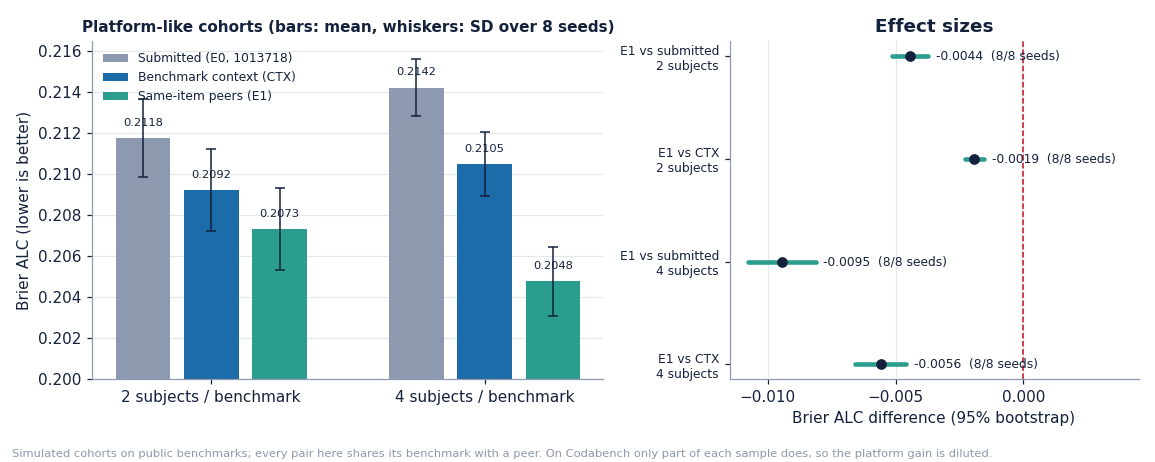
\includegraphics[width=\linewidth]{fig5_e1_item_peer.png}
\caption{E1 in platform-like cohorts. Left: Brier ALC per configuration (mean
and standard deviation over eight seeds). Right: held-out differences with
95\% component-bootstrap intervals.}
\label{fig:e1}
\end{figure}

\paragraph{Result.} E1 is accepted (Table~\ref{tab:e1}, Figure~\ref{fig:e1}).
The gain over the context rule is larger with more subjects per benchmark, as
expected if it comes from same-item evidence. Residuals alone, without the
context prior, are not better than the context rule with two subjects; both
parts are needed. The shipped \texttt{model.py} reproduces the simulator's
scores exactly (216 pair curves, maximum error zero) and returns exactly the
original rule's probabilities when only the target subject's labels exist
(2,220 checks). It passes the official \texttt{check\_submission\_zip.py}.

\paragraph{Expected size on the platform.} Every simulated pair shares its
benchmark with a peer. In the one Codabench sample we have seen, four of nine
pairs did. If that fraction is typical, the platform gain is about
$0.44\times0.0044\approx0.002$ Brier ALC against the submitted rule; this is an
arithmetic projection, not a measurement.

\section{Official Codabench results}
\begin{table}[t]
\centering\small
\caption{Codabench formative feedback (phase ``Competition'', task
``Amortized Prediction''). Each submission is scored on a newly sampled set of
nine subject--benchmark pairs; across-pair standard error of the mean is about
0.022, so these numbers check execution, not the difference between methods.}
\label{tab:codabench}
\begin{tabular}{rlrrr}
\toprule
ID & Archive & Pairs & Brier ALC & ECE\\
\midrule
1013718 & \texttt{submission\_original.zip} (Beta--Binomial) & 9 & 0.208365 & 0.136929\\
1015136 & \texttt{submission\_item\_peer.zip} (E1) & \CBPAIRS{} & \CBEONE{} & \CBECE{}\\
\bottomrule
\end{tabular}
\end{table}
Both archives ran to completion (Table~\ref{tab:codabench}). For submission
1013718, the formative Brier at budgets 0, 1, 3, 7, 15 and 31, averaged over its
nine pairs, was 0.2500, 0.2284, 0.2142, 0.1975, 0.1869 and 0.1796. The
per-pair tables are committed with the code. Submission 1015136 was scored on a different sample of eight pairs on seven benchmarks, one of which carried two subjects; its budget means were 0.2500, 0.2143, 0.1779, 0.1663, 0.1620 and 0.1599. The gap between the two formative scores is about one standard error and comes mostly from different pairs, so it is not evidence for E1. Our selected submission for final
evaluation is 1015136, the method of Section~\ref{sec:e1}; it falls back exactly to the
rule of 1013718 whenever no peer evidence is supplied.

\section{Inference, limitations, and reproducibility}
We average the eight seeds within each pair, then bootstrap 10,000 complete
content components. Each replicate recomputes total score difference divided
by total pair count, preserving the official pair-weighted estimand rather
than silently averaging benchmark means. Reported 95\% intervals are
descriptive; family-adjusted intervals are used when comparing promoted
candidate families. The grouped sign-randomization calculation uses a
plus-one correction and requires symmetry assumptions; it is not treated
as an exact distribution-free statement about transfer.

This bootstrap conditions on fitted cross-validation models; it does not
retrain the whole selection process for each replicate. Exact content hashes
do not catch paraphrases or every family relationship. Public-population
weights may differ from the platform's subject sampling, and binary outcomes
have heterogeneous meanings across released benchmarks. The inner validation
sets and folds can be imbalanced by a few large benchmarks. Fitted models
are not refitted on fit plus validation after selection, which is valid but
may sacrifice efficiency. We make no claim to exhaust model classes or
the potential value of pretrained representations.

The cohort simulator makes assumptions we could not check: the platform's
subject sampling, the share of items that two sampled subjects have in common,
and the use of one Bernoulli draw for an item with several recorded responses.
Cohorts were built only from items attempted by every member, which favours
same-item evidence; Section~\ref{sec:e1} gives the diluted projection. The
private test benchmarks are disjoint from all public data, so the size of the
transfer is unknown. E1 never uses an unrevealed label, a hidden identifier or
cross-call state; it reads only the \texttt{labeled} argument of the current call.

\paragraph{How to rerun.} The repository README lists every command. In short:
\texttt{python audit/download\_pinned.py --data DIR} fetches the 890 pinned files
(5.35 GB) and checks their SHA-256; \texttt{audit/build\_independent.py} builds
the 13,200 pairs; \texttt{audit/evaluate\_independent.py} and
\texttt{audit/evaluate\_context.py} produce Tables~\ref{tab:initial}
and~\ref{tab:context}; \texttt{experiments/E1/run\_e1.py 2} and \texttt{4}
produce Table~\ref{tab:e1} from the per-item cache in about one minute on a CPU,
and \texttt{experiments/E1/parity\_e1.py} checks the shipped predictor against
the simulator. \texttt{build/} regenerates every figure and animation. Package
versions are pinned in \texttt{requirements.txt} and
\texttt{experiments/E1/requirements-e1.lock}. No GPU, network access at scoring
time or paid inference is needed.

Code, protocols, results, the three submission archives and the formative
feedback are public at \url{https://github.com/Agnuxo1/AIMS-PAIEC-2026} under
the MIT licence; benchmark data keep their upstream licences and are not
redistributed. The initial release is tagged \texttt{v1.0.0}; this report
corresponds to release \texttt{v2.0.0}.

\paragraph{Training data and disclosure.} The only data used for development
are the public releases of the permitted measurement database at revision
\texttt{54074453}~\cite{data}; no other source, no private test data and no
paid inference were used, and the predictors fit nothing at scoring time.
LLM-based coding assistants (Anthropic Claude, including Claude Code) were used
for code, analysis scripts and writing, and as independent reviewers that did
not see new scores before their review. All numbers were produced by
deterministic scripts committed with the paper. Process failures are retained:
one replication attempt assumed a hash-group output order, two checks needed
JSON and floating-point fixes, and the first E1 analysis call failed on a
column-name format and was re-run on unchanged simulation outputs. The earlier
technical report withdrew a bootstrap interval without a reproducible generator.
The same author previously developed the BenchClaw benchmarking tools; no code
from them is used here.

\begin{thebibliography}{3}
\bibitem{competition} Stanford AIMS. Predictive AI Evaluation Competition at NeurIPS 2026.
\url{https://aims.stanford.edu/competition/}. Accessed 28 October 2026.
\bibitem{data} AIMS Foundations. Measurement database, frozen revision
\texttt{54074453}. \url{https://huggingface.co/datasets/aims-foundations/measurement-db}.
\bibitem{baseline} AIMS Foundations. PAIEC predictor baselines.
\url{https://github.com/aims-foundations/paiec_baseline}.
\end{thebibliography}
\end{document}
